%==============================================================================
%== template for LATEX poster =================================================
%==============================================================================
%
%--A0 beamer slide-------------------------------------------------------------
\documentclass[final]{beamer}\usepackage[]{graphicx}\usepackage[]{xcolor}
% maxwidth is the original width if it is less than linewidth
% otherwise use linewidth (to make sure the graphics do not exceed the margin)
\makeatletter
\def\maxwidth{ %
  \ifdim\Gin@nat@width>\linewidth
    \linewidth
  \else
    \Gin@nat@width
  \fi
}
\makeatother

\definecolor{fgcolor}{rgb}{0.345, 0.345, 0.345}
\newcommand{\hlnum}[1]{\textcolor[rgb]{0.686,0.059,0.569}{#1}}%
\newcommand{\hlstr}[1]{\textcolor[rgb]{0.192,0.494,0.8}{#1}}%
\newcommand{\hlcom}[1]{\textcolor[rgb]{0.678,0.584,0.686}{\textit{#1}}}%
\newcommand{\hlopt}[1]{\textcolor[rgb]{0,0,0}{#1}}%
\newcommand{\hlstd}[1]{\textcolor[rgb]{0.345,0.345,0.345}{#1}}%
\newcommand{\hlkwa}[1]{\textcolor[rgb]{0.161,0.373,0.58}{\textbf{#1}}}%
\newcommand{\hlkwb}[1]{\textcolor[rgb]{0.69,0.353,0.396}{#1}}%
\newcommand{\hlkwc}[1]{\textcolor[rgb]{0.333,0.667,0.333}{#1}}%
\newcommand{\hlkwd}[1]{\textcolor[rgb]{0.737,0.353,0.396}{\textbf{#1}}}%
\let\hlipl\hlkwb

\usepackage{framed}
\makeatletter
\newenvironment{kframe}{%
 \def\at@end@of@kframe{}%
 \ifinner\ifhmode%
  \def\at@end@of@kframe{\end{minipage}}%
  \begin{minipage}{\columnwidth}%
 \fi\fi%
 \def\FrameCommand##1{\hskip\@totalleftmargin \hskip-\fboxsep
 \colorbox{shadecolor}{##1}\hskip-\fboxsep
     % There is no \\@totalrightmargin, so:
     \hskip-\linewidth \hskip-\@totalleftmargin \hskip\columnwidth}%
 \MakeFramed {\advance\hsize-\width
   \@totalleftmargin\z@ \linewidth\hsize
   \@setminipage}}%
 {\par\unskip\endMakeFramed%
 \at@end@of@kframe}
\makeatother

\definecolor{shadecolor}{rgb}{.97, .97, .97}
\definecolor{messagecolor}{rgb}{0, 0, 0}
\definecolor{warningcolor}{rgb}{1, 0, 1}
\definecolor{errorcolor}{rgb}{1, 0, 0}
\newenvironment{knitrout}{}{} % an empty environment to be redefined in TeX

\usepackage{alltt}
\usepackage[orientation=portrait,
            size=custom,
            width=91.44,
            height=152.4,
            scale=1.5         % font scale factor
           ]{beamerposter}

\geometry{
  hmargin=2.5cm, % little modification of margins
}

%
\usepackage[utf8]{inputenc}

\newcommand{\dataset}{{\cal D}}

\linespread{1.05}
%
%==The poster style============================================================
\usetheme{sharelatex}

%==Title, date and authors of the poster=======================================
\title
[Wake Forest Biomedical Informatics Colloquium 2022] % Conference
{ % Poster title
Accelerated and interpretable oblique random survival forests
}

\author{ % Authors
Byron C. Jaeger\inst{1}, Sawyer Welden\inst{1}, Kristin Lenoir\inst{1}, Jaime L. Speiser\inst{1}, Matthew W. Segar\inst{2}, Ambarish Pandey\inst{3}, and Nicholas M. Pajewski\inst{1}
}
\institute
[Wake Forest University School of Medicine] % General University
{
\inst{1} Wake Forest University School of Medicine, Winston-Salem NC\\[0.3ex]
\inst{2} Texas Heart Institute, Houston TX\\[0.3ex]
\inst{3} University of Texas Southwestern Medical Center, Dallas TX
}
\date{September 23, 2022}
\IfFileExists{upquote.sty}{\usepackage{upquote}}{}
\begin{document}
\begin{frame}[t]
%==============================================================================
\begin{multicols}{3}
%==============================================================================
%==The poster content==========================================================
%==============================================================================

\section{Introduction}

\begin{itemize}

\item Risk prediction may reduce disease burden by guiding strategies for prevention and treatment.

\item Oblique random survival forests (RSFs) have high prediction accuracy, but also have high computational overhead and few methods for interpretation.\cite{ref1}

\item We developed methods to make oblique RSFs faster and more interpretable.

\end{itemize}

% In Ref.~\cite{ref1}...
% In Refs.~\cite{ref1,ref2}...
% On webpage~\cite{web}...


\section{Background}

\subsection{Axis-based and oblique trees}

Decision trees grow by splitting a set of training data into two subsets with maximally different expected outcomes. When the new subsets are formed based on \emph{a single predictor}, the tree is \textbf{axis-based} because the splits of the data are perpendicular to the axis of the predictor. When subsets are formed based on \textbf{a linear combination of predictors}, the tree is \textbf{oblique} because the splits are neither parallel nor perpendicular to the axis.

\vskip1ex
\begin{figure}
\centering
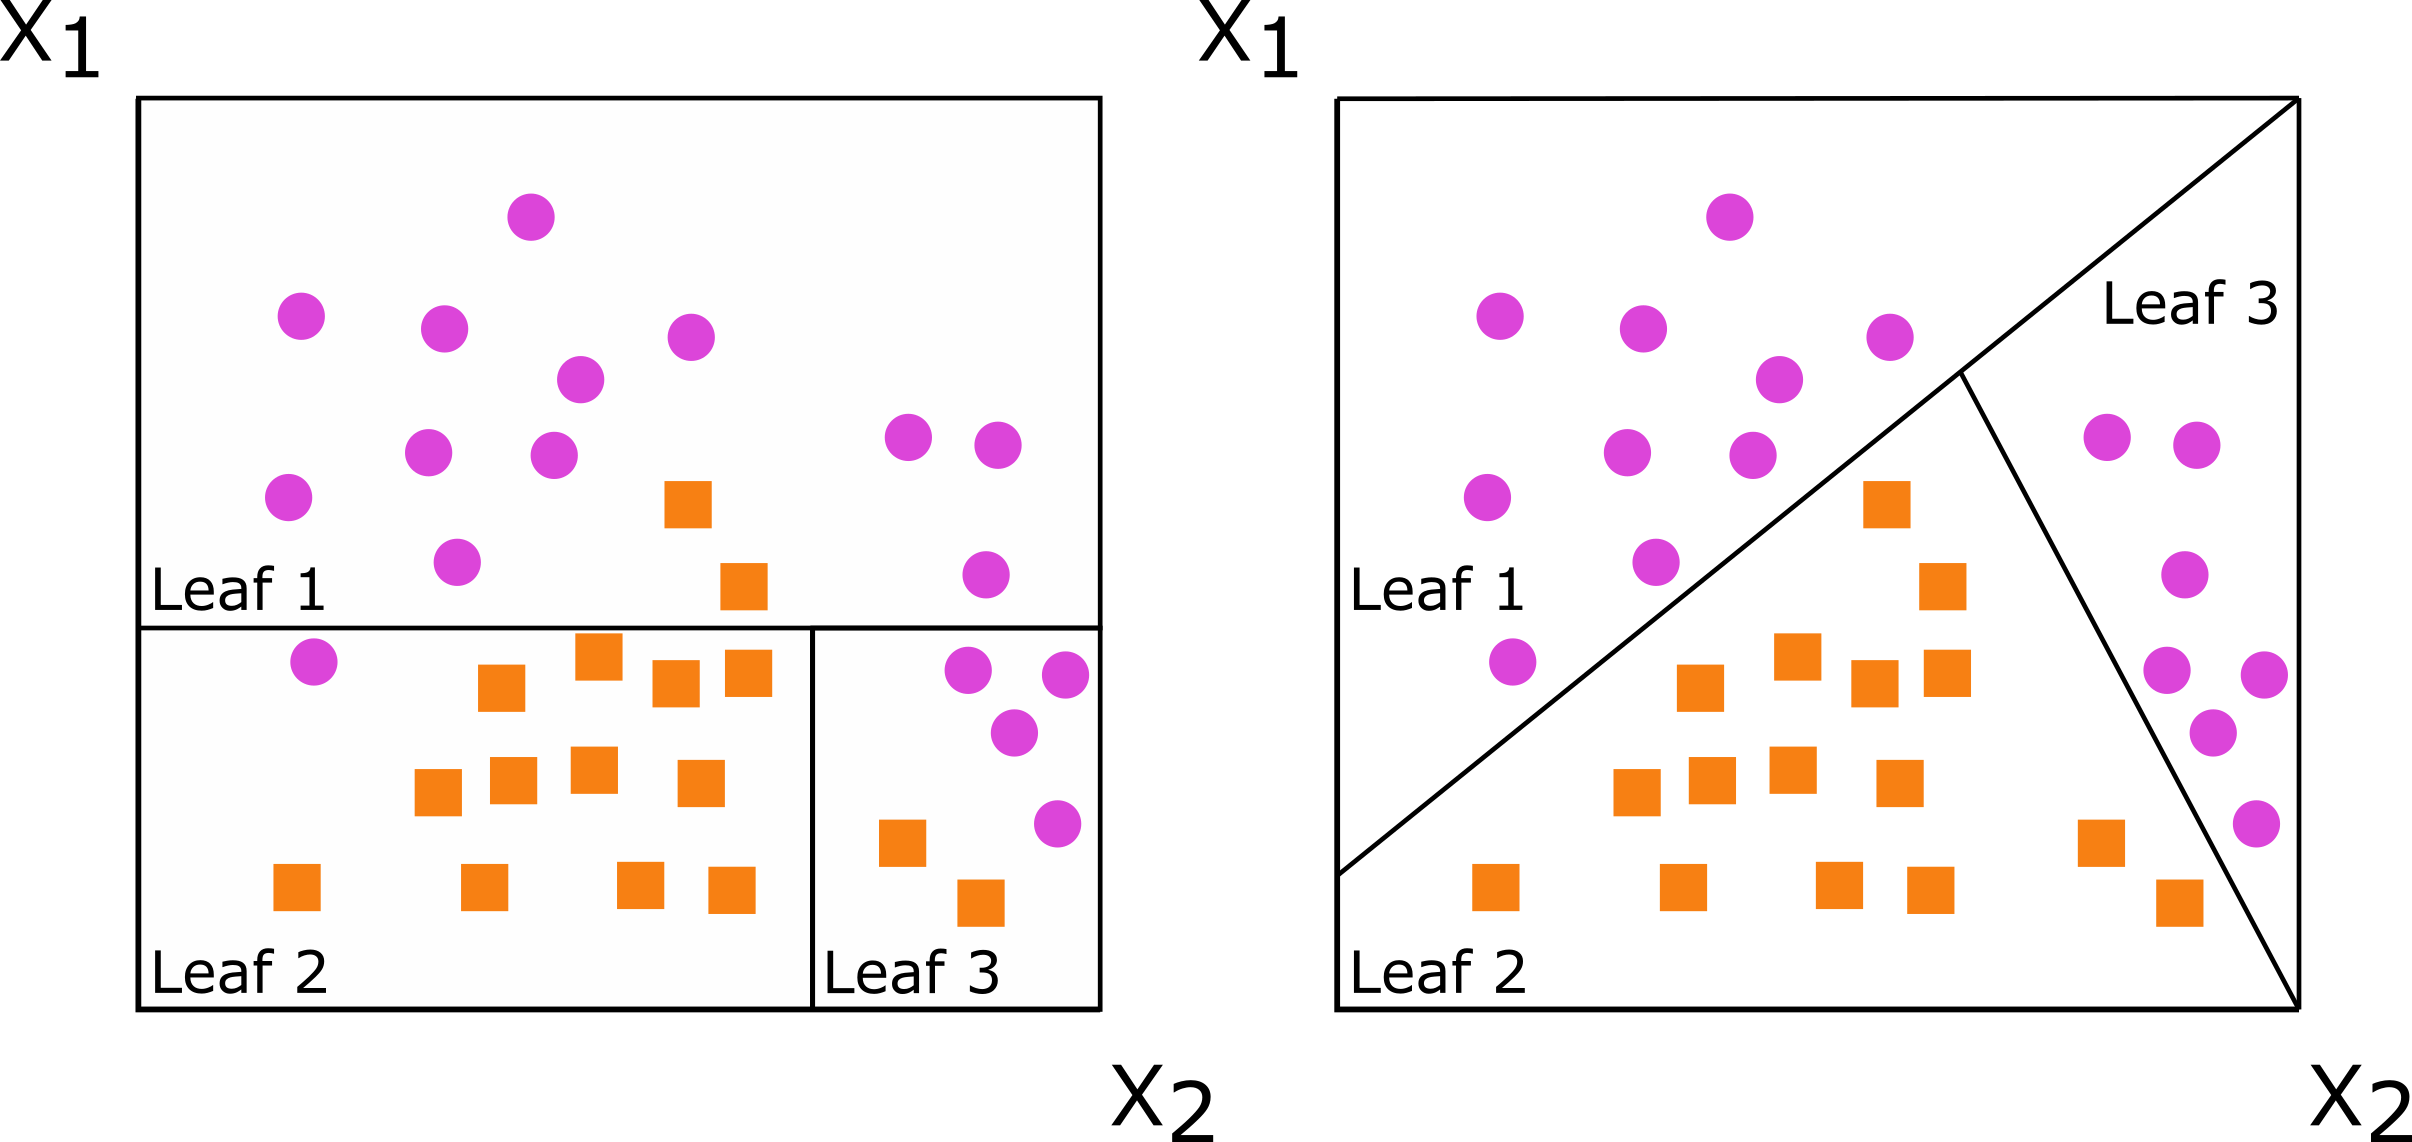
\includegraphics[width=0.99\columnwidth]{tree_axis_v_oblique.png}
\caption{Decision trees with axis-based splitting (left) and oblique splitting (right). The oblique trees do a better job of separating the two classes.}
\end{figure}
\vskip2ex

\textbf{Problems}: \begin{itemize}

\item Oblique RSFs have high computational overhead due to the large number of possible oblique splits to search through.

\item Oblique RSFs are difficult to interpret as there are few methods to estimate predictor importance using an oblique RSF.

\end{itemize}

\subsection{Standard technique for predictor importance: permutation}

\textbf{Definition}: For predictor $X$, the increase in prediction error after $X$ is randomly permuted.

\textbf{Problem}: Permuting a predictor does not account for the size of coefficients attached to it in linear combinations. In oblique random forests, important predictors are likely to have larger coefficients, and ignoring this leads to unreliable importance estimates.

\section{Accelerating the oblique random survival forest}

\subsection{Partial Newton Raphson scoring}

% Consider the usual framework for right-censored time-to-event outcomes. Let $\dataset_{\text{train}} = \left\{ (T_i, \delta_i, x_{i}) \right\}_{i=1}^{N_{\text{train}}}.$ Here, $T_i$ is the event time if $\delta_i=1$ or the censoring time if $\delta_i=0$, and $x_i$ is a vector of predictors values.

We propose to identify linear combinations of predictors in non-leaf nodes by applying Newton Raphson scoring to the partial Cox likelihood.

% \begin{equation}\label{eqn:cox-partial-likelihood}
% L(\beta) = \prod_{i=1}^m \frac{e^{x_{j(i)}^T \beta}}{\sum_{j \in R_i} e^{x_j^T \beta}},
% \end{equation}
% where $R_i$ is the set of indices, $j$, with $T_j \geq t_i$ (those still at risk at time $t_i$), and $j(i)$ is the index of the observation for which an event occurred at time $t_i$.

\textbf{Hypothesis}: Using one Newton Raphson iteration to identify linear combinations of predictors will yield an efficient oblique RSF with no loss of prediction accuracy compared to other learners: \begin{itemize}

\item \texttt{aorsf-fast}: One Newton Raphson iteration

\item \texttt{aorsf-cph}: Newton Raphson until convergence (\emph{i.e.}, fits a Cox proportional hazards model)

\item \texttt{obliqueRSF}: Penalized regression (\emph{i.e.}, the original method used for oblique RSFs)

\item Many other learners (see ArXiv paper for full description - QR code is in the references)

\end{itemize}

\vskip3ex

\section{Introducing negation importance}

\textbf{Definition}: For predictor $X$, the increase in an oblique random forest's prediction error after coefficients attached to $X$ are multiplied by -1.

\textbf{Hypothesis}: negation importance will improve detection of signal versus noise predictors.

\section{Benchmarks}

\subsection{Prediction accuracy}

We evaluated \texttt{aorsf-fast}'s Discrimination (C-statistic) compared to several machine learning algorithms in 35 distinct risk prediction tasks drawn from 21 distinct datasets. Using Bayesian mixed models, inferences on equivalence and inferiority of \texttt{aorsf-fast} versus other learners were made.

\vskip1ex
\begin{figure}
\centering
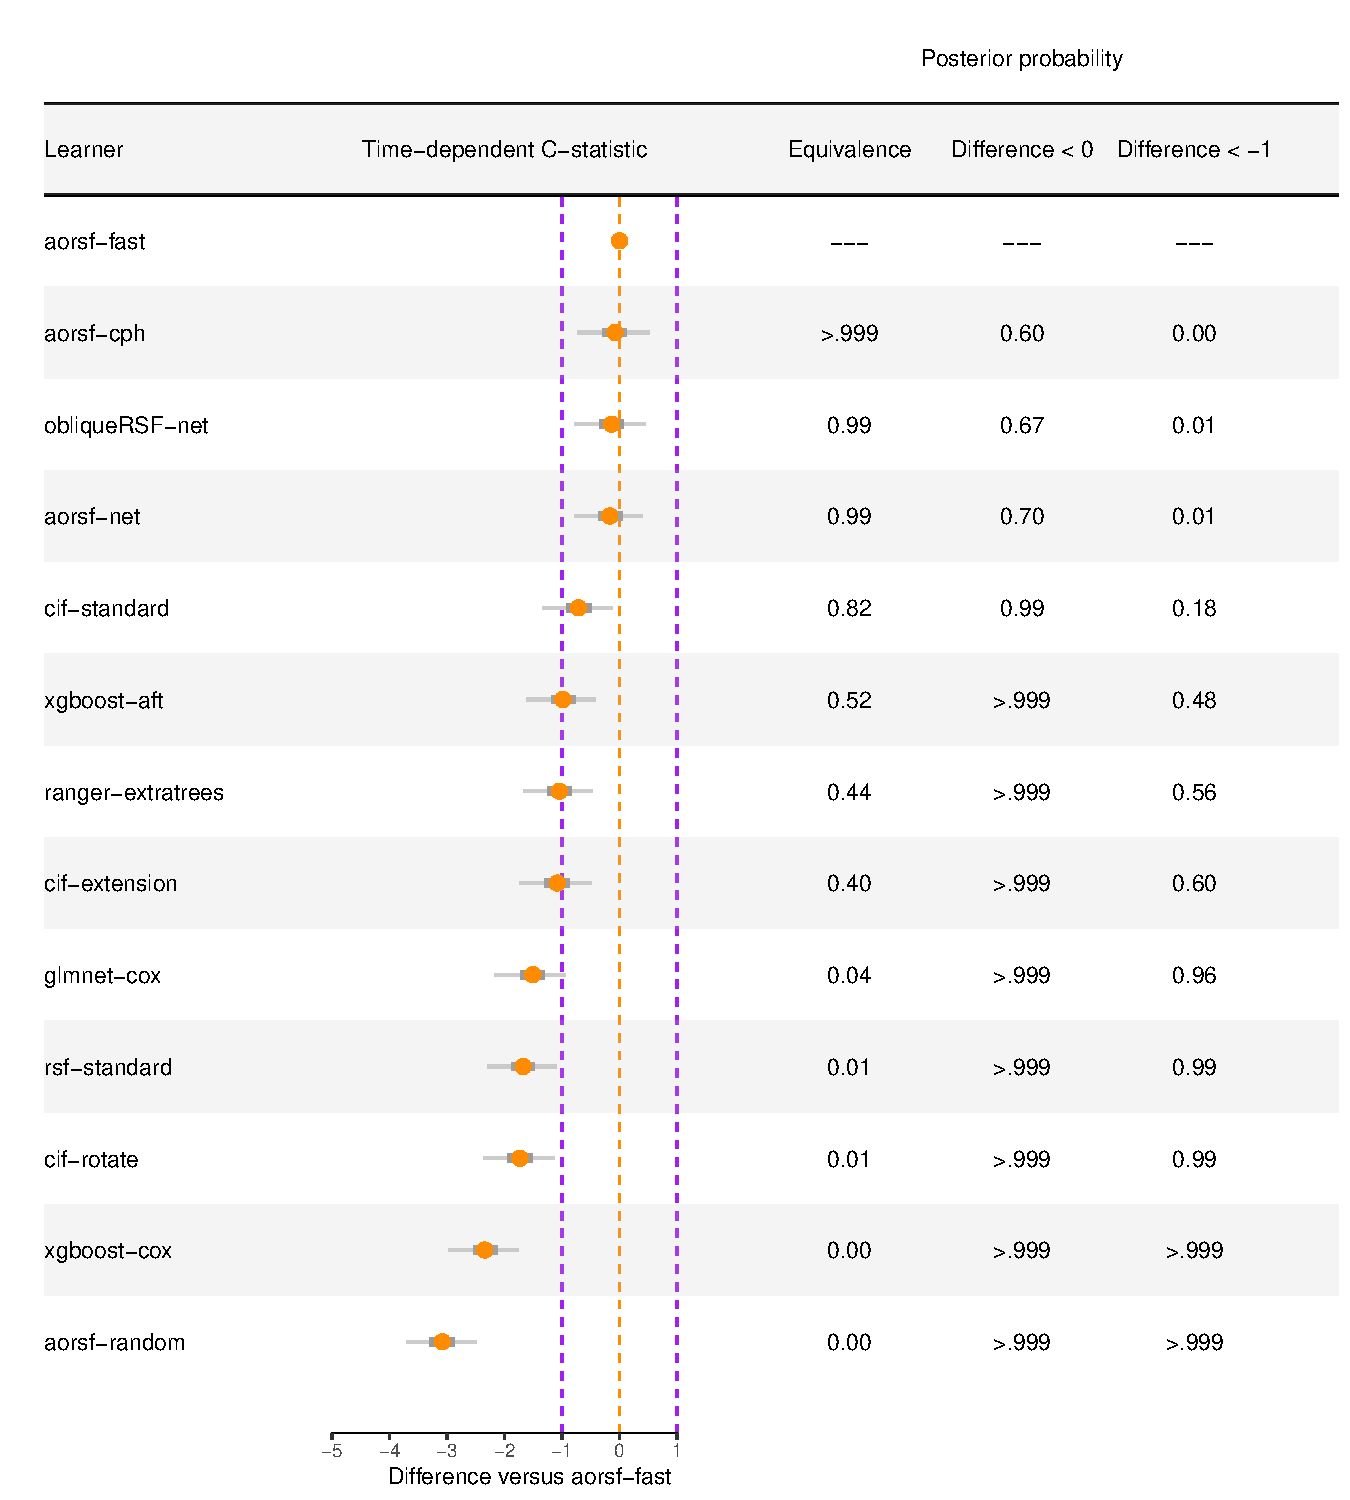
\includegraphics[width=0.99\columnwidth]{bm_pred_model_viz_cstat-1.pdf}
\caption{Expected differences in C-statistic between \texttt{aorsf-fast} and other learners. A region of practical equivalence is shown by purple lines, and a boundary of non-zero difference is shown by an orange line.}
\end{figure}
\vskip2ex

\subsection{Predictor importance}

We evaluated negation importance and several other methods based on how well they discriminated between relevant and irrelevant predictors in a simulation study. In addition to negation, we considered \begin{itemize}

\item ANOVA importance: the proportion of times a given predictor's p-value is <0.001 in linear combinations

\item Permutation importance: increase in prediction error after a given predictor is randomly permuted.

\item Shapley importance: the expected absolute contribution of a predictor to a model's predictions.

\end{itemize}

\vskip1ex
\begin{figure}
\centering
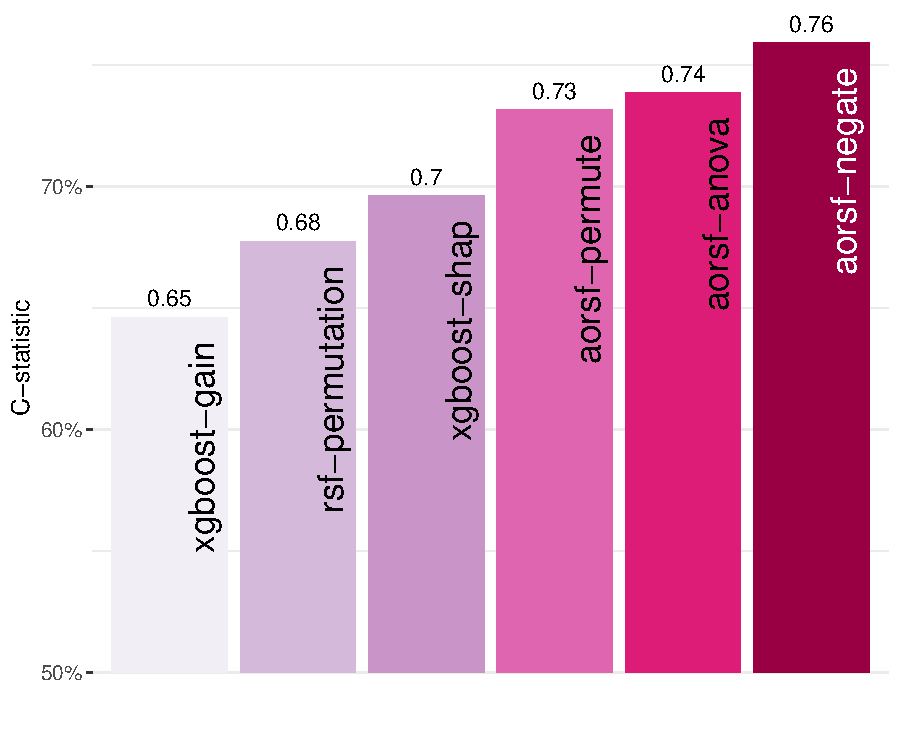
\includegraphics[width=0.99\columnwidth]{fig_vi_smry.pdf}
\caption{C-statistic for variable selection using different techniques to estimate predictor importance.}
\end{figure}
\vskip2ex

\subsection{Computational efficiency}

We evaluated the computational efficiency of the \texttt{aorsf-fast} compared to other machine learning algorithms.


\vskip1ex
\begin{figure}
\centering
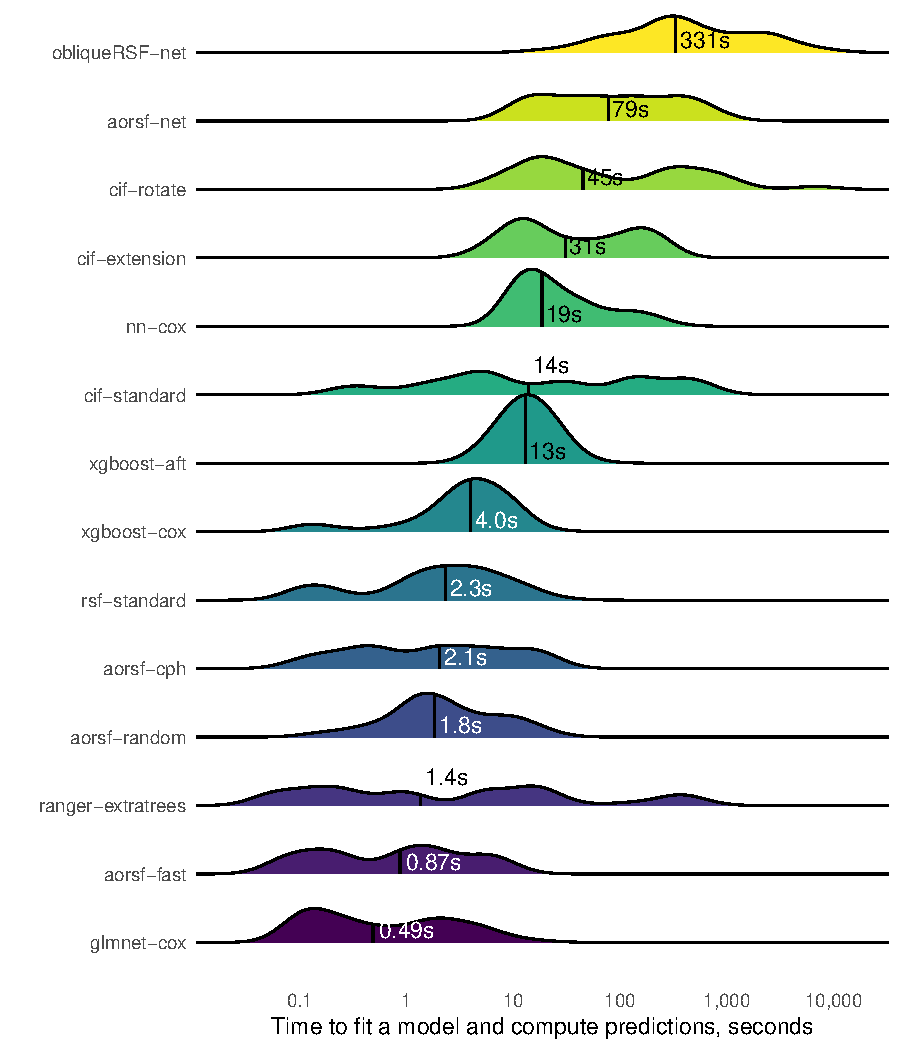
\includegraphics[width=0.99\columnwidth]{fig_pred_time.pdf}
\caption{Distribution of time taken to fit a prediction model and compute predicted risk. The median time, in seconds, is printed for each learner}
\end{figure}
\vskip2ex

\section{Summary and conclusions}

\begin{itemize}

\item Oblique RSFs have exceptional prediction accuracy.

\item We have developed a method to fit oblique RSFs efficiently, with no loss of prediction accuracy.

\item We have also introduced a general method to estimate predictor importance with oblique random forests (not just RSFs), and demonstrated its effectiveness specifically for the oblique RSF.

\end{itemize}

\subsection{Acknowledgments}

Research reported in this publication was supported by the Center for Biomedical Informatics, Wake Forest University School of Medicine. The project described was supported by the National Center for Advancing Translational Sciences (NCATS), National Institutes of Health, through Grant Award Number UL1TR001420. The content is solely the responsibility of the authors and does not necessarily represent the official views of the NIH.


%==============================================================================
%==End of content==============================================================
%==============================================================================

%--References------------------------------------------------------------------

\subsection{References}

\vskip1ex
\begin{center}

\includegraphics[width=0.4\columnwidth]{aorsf-package.png}
\hspace{1cm}

\includegraphics[width=0.4\columnwidth]{aorsf-arxiv.png}
\end{center}

\begin{thebibliography}{99}

\bibitem{ref1} Jaeger, Byron C., et al. ``Oblique random survival forests." \emph{The Annals of Applied Statistics} 13.3 (2019): 1847-1883.



\end{thebibliography}
%--End of references-----------------------------------------------------------

\end{multicols}

%==============================================================================
\end{frame}
\end{document}
